\documentclass[twoside]{book}

% Packages required by doxygen
\usepackage{fixltx2e}
\usepackage{calc}
\usepackage{doxygen}
\usepackage[export]{adjustbox} % also loads graphicx
\usepackage{graphicx}
\usepackage[utf8]{inputenc}
\usepackage{makeidx}
\usepackage{multicol}
\usepackage{multirow}
\PassOptionsToPackage{warn}{textcomp}
\usepackage{textcomp}
\usepackage[nointegrals]{wasysym}
\usepackage[table]{xcolor}

% Font selection
\usepackage[T1]{fontenc}
\usepackage[scaled=.90]{helvet}
\usepackage{courier}
\usepackage{amssymb}
\usepackage{sectsty}
\renewcommand{\familydefault}{\sfdefault}
\allsectionsfont{%
  \fontseries{bc}\selectfont%
  \color{darkgray}%
}
\renewcommand{\DoxyLabelFont}{%
  \fontseries{bc}\selectfont%
  \color{darkgray}%
}
\newcommand{\+}{\discretionary{\mbox{\scriptsize$\hookleftarrow$}}{}{}}

% Page & text layout
\usepackage{geometry}
\geometry{%
  a4paper,%
  top=2.5cm,%
  bottom=2.5cm,%
  left=2.5cm,%
  right=2.5cm%
}
\tolerance=750
\hfuzz=15pt
\hbadness=750
\setlength{\emergencystretch}{15pt}
\setlength{\parindent}{0cm}
\setlength{\parskip}{3ex plus 2ex minus 2ex}
\makeatletter
\renewcommand{\paragraph}{%
  \@startsection{paragraph}{4}{0ex}{-1.0ex}{1.0ex}{%
    \normalfont\normalsize\bfseries\SS@parafont%
  }%
}
\renewcommand{\subparagraph}{%
  \@startsection{subparagraph}{5}{0ex}{-1.0ex}{1.0ex}{%
    \normalfont\normalsize\bfseries\SS@subparafont%
  }%
}
\makeatother

% Headers & footers
\usepackage{fancyhdr}
\pagestyle{fancyplain}
\fancyhead[LE]{\fancyplain{}{\bfseries\thepage}}
\fancyhead[CE]{\fancyplain{}{}}
\fancyhead[RE]{\fancyplain{}{\bfseries\leftmark}}
\fancyhead[LO]{\fancyplain{}{\bfseries\rightmark}}
\fancyhead[CO]{\fancyplain{}{}}
\fancyhead[RO]{\fancyplain{}{\bfseries\thepage}}
\fancyfoot[LE]{\fancyplain{}{}}
\fancyfoot[CE]{\fancyplain{}{}}
\fancyfoot[RE]{\fancyplain{}{\bfseries\scriptsize Generated by Doxygen }}
\fancyfoot[LO]{\fancyplain{}{\bfseries\scriptsize Generated by Doxygen }}
\fancyfoot[CO]{\fancyplain{}{}}
\fancyfoot[RO]{\fancyplain{}{}}
\renewcommand{\footrulewidth}{0.4pt}
\renewcommand{\chaptermark}[1]{%
  \markboth{#1}{}%
}
\renewcommand{\sectionmark}[1]{%
  \markright{\thesection\ #1}%
}

% Indices & bibliography
\usepackage{natbib}
\usepackage[titles]{tocloft}
\setcounter{tocdepth}{3}
\setcounter{secnumdepth}{5}
\makeindex

% Hyperlinks (required, but should be loaded last)
\usepackage{ifpdf}
\ifpdf
  \usepackage[pdftex,pagebackref=true]{hyperref}
\else
  \usepackage[ps2pdf,pagebackref=true]{hyperref}
\fi
\hypersetup{%
  colorlinks=true,%
  linkcolor=blue,%
  citecolor=blue,%
  unicode%
}

% Custom commands
\newcommand{\clearemptydoublepage}{%
  \newpage{\pagestyle{empty}\cleardoublepage}%
}

\usepackage{caption}
\captionsetup{labelsep=space,justification=centering,font={bf},singlelinecheck=off,skip=4pt,position=top}

%===== C O N T E N T S =====

\begin{document}

% Titlepage & ToC
\hypersetup{pageanchor=false,
             bookmarksnumbered=true,
             pdfencoding=unicode
            }
\pagenumbering{alph}
\begin{titlepage}
\vspace*{7cm}
\begin{center}%
{\Large Le Jeu de la Vie \\[1ex]\large v4.\+0 }\\
\vspace*{1cm}
{\large Generated by Doxygen 1.8.13}\\
\end{center}
\end{titlepage}
\clearemptydoublepage
\pagenumbering{roman}
\tableofcontents
\clearemptydoublepage
\pagenumbering{arabic}
\hypersetup{pageanchor=true}

%--- Begin generated contents ---
\chapter{File Index}
\section{File List}
Here is a list of all documented files with brief descriptions\+:\begin{DoxyCompactList}
\item\contentsline{section}{src/\hyperlink{grille_8c}{grille.\+c} \\*Fichier \hyperlink{grille_8c}{grille.\+c} }{\pageref{grille_8c}}{}
\item\contentsline{section}{src/\hyperlink{io_8c}{io.\+c} \\*Fichier \hyperlink{io_8c}{io.\+c} }{\pageref{io_8c}}{}
\item\contentsline{section}{src/\hyperlink{jeu_8c}{jeu.\+c} \\*Fichier \hyperlink{jeu_8c}{jeu.\+c} }{\pageref{jeu_8c}}{}
\item\contentsline{section}{src/\hyperlink{main_8c}{main.\+c} \\*Fichier \hyperlink{main_8c}{main.\+c} (coeur) }{\pageref{main_8c}}{}
\end{DoxyCompactList}

\chapter{File Documentation}
\hypertarget{graphic__io_8c}{}\section{src/graphic\+\_\+io.c File Reference}
\label{graphic__io_8c}\index{src/graphic\+\_\+io.\+c@{src/graphic\+\_\+io.\+c}}


\hyperlink{io_8c}{io.\+c} version graphique  


{\ttfamily \#include \char`\"{}../include/io.\+h\char`\"{}}\newline
{\ttfamily \#include $<$string.\+h$>$}\newline
{\ttfamily \#include $<$cairo.\+h$>$}\newline
{\ttfamily \#include $<$cairo-\/xlib.\+h$>$}\newline
{\ttfamily \#include $<$X11/\+Xlib.\+h$>$}\newline
{\ttfamily \#include $<$X11/\+Xutil.\+h$>$}\newline
{\ttfamily \#include $<$X11/\+Xos.\+h$>$}\newline
Include dependency graph for graphic\+\_\+io.\+c\+:
\nopagebreak
\begin{figure}[H]
\begin{center}
\leavevmode
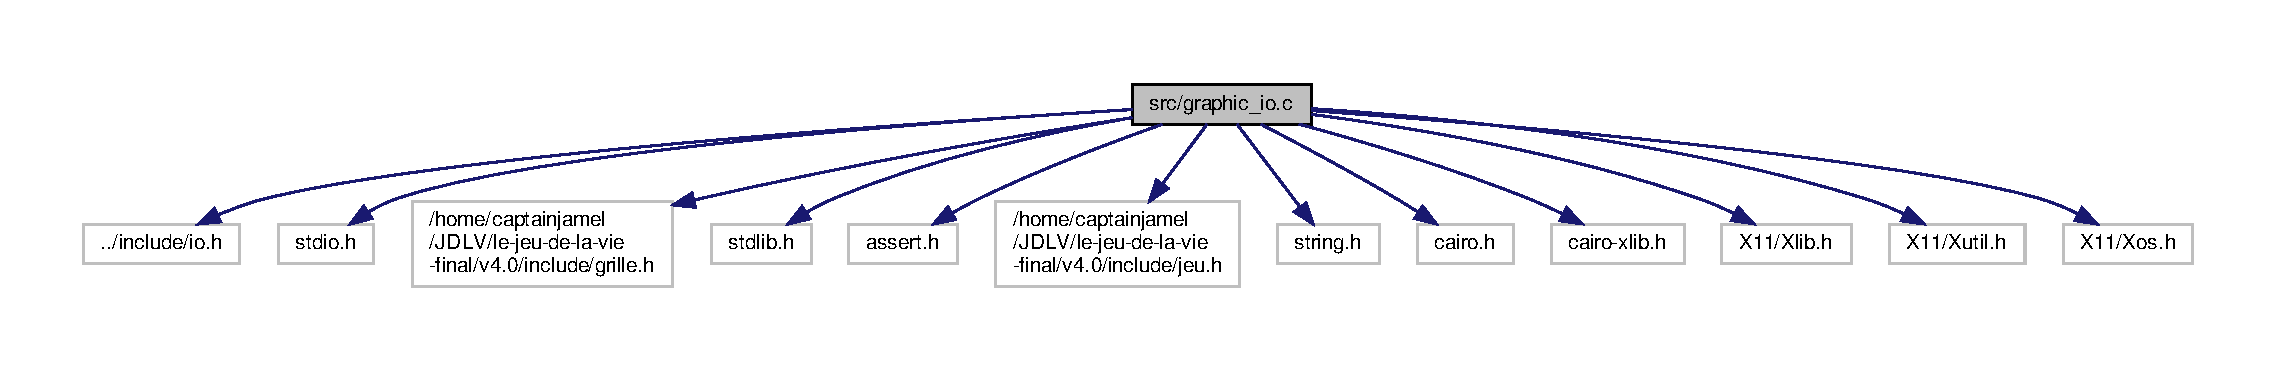
\includegraphics[width=350pt]{graphic__io_8c__incl}
\end{center}
\end{figure}
\subsection*{Functions}
\begin{DoxyCompactItemize}
\item 
\mbox{\Hypertarget{graphic__io_8c_af7a0e72638475403c88280d95e5e5ddc}\label{graphic__io_8c_af7a0e72638475403c88280d95e5e5ddc}} 
void {\bfseries affiche\+\_\+grille\+\_\+gr} (cairo\+\_\+surface\+\_\+t $\ast$surface, grille g)
\item 
\mbox{\Hypertarget{graphic__io_8c_a88493b3c55828670e47150a95ed7db5b}\label{graphic__io_8c_a88493b3c55828670e47150a95ed7db5b}} 
void {\bfseries debut\+\_\+jeu} (grille $\ast$g, grille $\ast$gc)
\end{DoxyCompactItemize}
\subsection*{Variables}
\begin{DoxyCompactItemize}
\item 
\mbox{\Hypertarget{graphic__io_8c_ae0aa920346296038f211a227948cc303}\label{graphic__io_8c_ae0aa920346296038f211a227948cc303}} 
char {\bfseries char\+Evol} \mbox{[}20\mbox{]}
\item 
\mbox{\Hypertarget{graphic__io_8c_ab9f5d45c98b073e219011d616152beef}\label{graphic__io_8c_ab9f5d45c98b073e219011d616152beef}} 
char {\bfseries text\+Evol} \mbox{[}50\mbox{]}
\item 
\mbox{\Hypertarget{graphic__io_8c_a0e9a30bb8b7641d7e0bb8da3389dc99d}\label{graphic__io_8c_a0e9a30bb8b7641d7e0bb8da3389dc99d}} 
char {\bfseries file\+Name} \mbox{[}1000\mbox{]}
\end{DoxyCompactItemize}


\subsection{Detailed Description}
\hyperlink{io_8c}{io.\+c} version graphique 


\hypertarget{grille_8c}{}\section{src/grille.c File Reference}
\label{grille_8c}\index{src/grille.\+c@{src/grille.\+c}}


Fichier \hyperlink{grille_8c}{grille.\+c}.  


{\ttfamily \#include \char`\"{}../include/grille.\+h\char`\"{}}\newline
Include dependency graph for grille.\+c\+:
\nopagebreak
\begin{figure}[H]
\begin{center}
\leavevmode
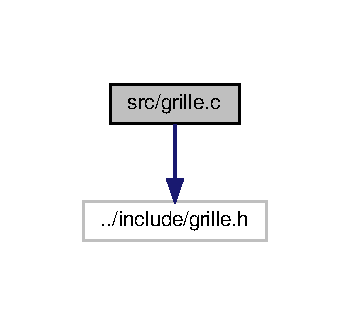
\includegraphics[width=350pt]{grille_8c__incl}
\end{center}
\end{figure}
\subsection*{Functions}
\begin{DoxyCompactItemize}
\item 
\mbox{\Hypertarget{grille_8c_ae621f51c60aa4fafaa0c9f6c9b5a4036}\label{grille_8c_ae621f51c60aa4fafaa0c9f6c9b5a4036}} 
void {\bfseries alloue\+\_\+grille} (int l, int c, grille $\ast$g)
\item 
\mbox{\Hypertarget{grille_8c_a7074b2b15576e9d2b3cd15c3a1dc7012}\label{grille_8c_a7074b2b15576e9d2b3cd15c3a1dc7012}} 
void {\bfseries libere\+\_\+grille} (grille $\ast$g)
\item 
\mbox{\Hypertarget{grille_8c_adf5501cc0bbad28f5ffc561d92197e4e}\label{grille_8c_adf5501cc0bbad28f5ffc561d92197e4e}} 
void {\bfseries init\+\_\+grille\+\_\+from\+\_\+file} (char $\ast$filename, grille $\ast$g)
\item 
\mbox{\Hypertarget{grille_8c_a63b3ae16c86b568f6aa8f9ce84128b1e}\label{grille_8c_a63b3ae16c86b568f6aa8f9ce84128b1e}} 
void {\bfseries copie\+\_\+grille} (grille gs, grille gd)
\end{DoxyCompactItemize}


\subsection{Detailed Description}
Fichier \hyperlink{grille_8c}{grille.\+c}. 


\hypertarget{io_8c}{}\section{io.\+c File Reference}
\label{io_8c}\index{io.\+c@{io.\+c}}


Fichier \hyperlink{io_8c}{io.\+c}.  


{\ttfamily \#include \char`\"{}io.\+h\char`\"{}}\\*
Include dependency graph for io.\+c\+:\nopagebreak
\begin{figure}[H]
\begin{center}
\leavevmode
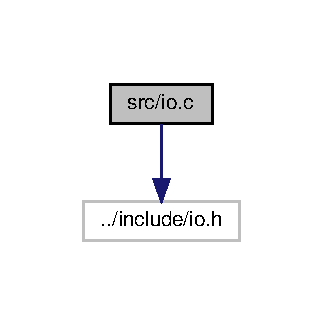
\includegraphics[width=262pt]{io_8c__incl}
\end{center}
\end{figure}
\subsection*{Functions}
\begin{DoxyCompactItemize}
\item 
void \hyperlink{io_8c_a1215302c999b838f742e37d46df4a2e6}{affiche\+\_\+evolution} (int $\ast$evol)
\begin{DoxyCompactList}\small\item\em affiche le temps d\textquotesingle{}évolution (incrémenté de 1 à chaque coup) \end{DoxyCompactList}\item 
void \hyperlink{io_8c_a634cf584c380ce221d5d4199f3e813bd}{affiche\+\_\+trait} (int c)
\begin{DoxyCompactList}\small\item\em Permet d\textquotesingle{}afficher le caractère \textquotesingle{}$\vert$\textquotesingle{} pour faire les traits. \end{DoxyCompactList}\item 
void \hyperlink{io_8c_a3f3ff78e56fcf21a932ff73b70635554}{affiche\+\_\+ligne} (int c, int $\ast$ligne)
\begin{DoxyCompactList}\small\item\em Affichage d\textquotesingle{}une ligne de la grille. \end{DoxyCompactList}\item 
void \hyperlink{io_8c_a90cb8ec05374b46d9995705ed4954f34}{affiche\+\_\+grille} (\hyperlink{structgrille}{grille} g)
\begin{DoxyCompactList}\small\item\em affichage d\textquotesingle{}une grille \end{DoxyCompactList}\item 
void \hyperlink{io_8c_ab36a6f8957cd3e682119007836ce6ad5}{efface\+\_\+grille} (\hyperlink{structgrille}{grille} g)
\begin{DoxyCompactList}\small\item\em effacement d\textquotesingle{}une grille \end{DoxyCompactList}\item 
void \hyperlink{io_8c_a88493b3c55828670e47150a95ed7db5b}{debut\+\_\+jeu} (\hyperlink{structgrille}{grille} $\ast$g, \hyperlink{structgrille}{grille} $\ast$gc)
\begin{DoxyCompactList}\small\item\em debute le jeu \end{DoxyCompactList}\end{DoxyCompactItemize}


\subsection{Detailed Description}
Fichier \hyperlink{io_8c}{io.\+c}. 



\subsection{Function Documentation}
\index{io.\+c@{io.\+c}!affiche\+\_\+evolution@{affiche\+\_\+evolution}}
\index{affiche\+\_\+evolution@{affiche\+\_\+evolution}!io.\+c@{io.\+c}}
\subsubsection[{\texorpdfstring{affiche\+\_\+evolution(int $\ast$evol)}{affiche_evolution(int *evol)}}]{\setlength{\rightskip}{0pt plus 5cm}void affiche\+\_\+evolution (
\begin{DoxyParamCaption}
\item[{int $\ast$}]{evol}
\end{DoxyParamCaption}
)}\hypertarget{io_8c_a1215302c999b838f742e37d46df4a2e6}{}\label{io_8c_a1215302c999b838f742e37d46df4a2e6}


affiche le temps d\textquotesingle{}évolution (incrémenté de 1 à chaque coup) 


\begin{DoxyParams}{Parameters}
{\em $\ast$evol} & pointeur sur la variable d\textquotesingle{}evolution \\
\hline
\end{DoxyParams}
\index{io.\+c@{io.\+c}!affiche\+\_\+grille@{affiche\+\_\+grille}}
\index{affiche\+\_\+grille@{affiche\+\_\+grille}!io.\+c@{io.\+c}}
\subsubsection[{\texorpdfstring{affiche\+\_\+grille(grille g)}{affiche_grille(grille g)}}]{\setlength{\rightskip}{0pt plus 5cm}void affiche\+\_\+grille (
\begin{DoxyParamCaption}
\item[{{\bf grille}}]{g}
\end{DoxyParamCaption}
)}\hypertarget{io_8c_a90cb8ec05374b46d9995705ed4954f34}{}\label{io_8c_a90cb8ec05374b46d9995705ed4954f34}


affichage d\textquotesingle{}une grille 


\begin{DoxyParams}{Parameters}
{\em g} & grille \\
\hline
\end{DoxyParams}
\index{io.\+c@{io.\+c}!affiche\+\_\+ligne@{affiche\+\_\+ligne}}
\index{affiche\+\_\+ligne@{affiche\+\_\+ligne}!io.\+c@{io.\+c}}
\subsubsection[{\texorpdfstring{affiche\+\_\+ligne(int c, int $\ast$ligne)}{affiche_ligne(int c, int *ligne)}}]{\setlength{\rightskip}{0pt plus 5cm}void affiche\+\_\+ligne (
\begin{DoxyParamCaption}
\item[{int}]{c, }
\item[{int $\ast$}]{ligne}
\end{DoxyParamCaption}
)}\hypertarget{io_8c_a3f3ff78e56fcf21a932ff73b70635554}{}\label{io_8c_a3f3ff78e56fcf21a932ff73b70635554}


Affichage d\textquotesingle{}une ligne de la grille. 


\begin{DoxyParams}{Parameters}
{\em c} & colonnes \\
\hline
{\em $\ast$ligne} & pointeur lignes \\
\hline
\end{DoxyParams}
\index{io.\+c@{io.\+c}!affiche\+\_\+trait@{affiche\+\_\+trait}}
\index{affiche\+\_\+trait@{affiche\+\_\+trait}!io.\+c@{io.\+c}}
\subsubsection[{\texorpdfstring{affiche\+\_\+trait(int c)}{affiche_trait(int c)}}]{\setlength{\rightskip}{0pt plus 5cm}void affiche\+\_\+trait (
\begin{DoxyParamCaption}
\item[{int}]{c}
\end{DoxyParamCaption}
)}\hypertarget{io_8c_a634cf584c380ce221d5d4199f3e813bd}{}\label{io_8c_a634cf584c380ce221d5d4199f3e813bd}


Permet d\textquotesingle{}afficher le caractère \textquotesingle{}$\vert$\textquotesingle{} pour faire les traits. 


\begin{DoxyParams}{Parameters}
{\em c} & colonnes \\
\hline
\end{DoxyParams}
\index{io.\+c@{io.\+c}!debut\+\_\+jeu@{debut\+\_\+jeu}}
\index{debut\+\_\+jeu@{debut\+\_\+jeu}!io.\+c@{io.\+c}}
\subsubsection[{\texorpdfstring{debut\+\_\+jeu(grille $\ast$g, grille $\ast$gc)}{debut_jeu(grille *g, grille *gc)}}]{\setlength{\rightskip}{0pt plus 5cm}void debut\+\_\+jeu (
\begin{DoxyParamCaption}
\item[{{\bf grille} $\ast$}]{g, }
\item[{{\bf grille} $\ast$}]{gc}
\end{DoxyParamCaption}
)}\hypertarget{io_8c_a88493b3c55828670e47150a95ed7db5b}{}\label{io_8c_a88493b3c55828670e47150a95ed7db5b}


debute le jeu 


\begin{DoxyParams}{Parameters}
{\em $\ast$g} & pointeur grille \\
\hline
{\em $\ast$gc} & pointeur grille On utilise cette fonction avec les touches \textquotesingle{}entrée\textquotesingle{} (avancer), \textquotesingle{}q\textquotesingle{} (quitter), \textquotesingle{}n\textquotesingle{} (changement de grille), \textquotesingle{}c\textquotesingle{} (cyclique-\/$>$non-\/cyclique) (niv2prototype) \\
\hline
\end{DoxyParams}
\index{io.\+c@{io.\+c}!efface\+\_\+grille@{efface\+\_\+grille}}
\index{efface\+\_\+grille@{efface\+\_\+grille}!io.\+c@{io.\+c}}
\subsubsection[{\texorpdfstring{efface\+\_\+grille(grille g)}{efface_grille(grille g)}}]{\setlength{\rightskip}{0pt plus 5cm}void efface\+\_\+grille (
\begin{DoxyParamCaption}
\item[{{\bf grille}}]{g}
\end{DoxyParamCaption}
)}\hypertarget{io_8c_ab36a6f8957cd3e682119007836ce6ad5}{}\label{io_8c_ab36a6f8957cd3e682119007836ce6ad5}


effacement d\textquotesingle{}une grille 


\begin{DoxyParams}{Parameters}
{\em g} & grille \\
\hline
\end{DoxyParams}

\hypertarget{jeu_8c}{}\section{jeu.\+c File Reference}
\label{jeu_8c}\index{jeu.\+c@{jeu.\+c}}


Fichier \hyperlink{jeu_8c}{jeu.\+c}.  


{\ttfamily \#include \char`\"{}jeu.\+h\char`\"{}}\\*
Include dependency graph for jeu.\+c\+:\nopagebreak
\begin{figure}[H]
\begin{center}
\leavevmode
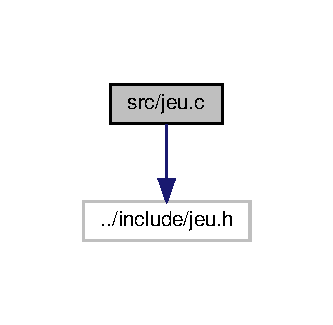
\includegraphics[width=262pt]{jeu_8c__incl}
\end{center}
\end{figure}
\subsection*{Functions}
\begin{DoxyCompactItemize}
\item 
int \hyperlink{jeu_8c_a59bc96faa8e7d7004fd8f342c0462b1d}{compte\+\_\+voisins\+\_\+vivants\+\_\+cycliques} (int i, int j, \hyperlink{structgrille}{grille} g)
\begin{DoxyCompactList}\small\item\em compte le nombre de voisins vivants de la cellule (i,j) les bords sont cycliques. \end{DoxyCompactList}\item 
int \hyperlink{jeu_8c_a1851122103353d1c8d18a4323683c087}{compte\+\_\+voisins\+\_\+vivants\+\_\+non\+\_\+cycliques} (int i, int j, \hyperlink{structgrille}{grille} g)
\begin{DoxyCompactList}\small\item\em compte le nombre de voisins vivant de la cellule (i,j) les bords ne sont pas cycliques. \end{DoxyCompactList}\item 
void \hyperlink{jeu_8c_a6c21b473d74c758d5c73a8a518a757d5}{evolue\+\_\+sv} (\hyperlink{structgrille}{grille} $\ast$g, \hyperlink{structgrille}{grille} $\ast$gc, int($\ast$cyclique\+\_\+ou\+\_\+pas)(int, int, \hyperlink{structgrille}{grille}))
\begin{DoxyCompactList}\small\item\em fait évoluer la grille g d\textquotesingle{}un pas de temps sans vieillissment \end{DoxyCompactList}\item 
void \hyperlink{jeu_8c_a87a51658c5ccfcf36921203d814080e7}{evolue\+\_\+v} (\hyperlink{structgrille}{grille} $\ast$g, \hyperlink{structgrille}{grille} $\ast$gc, int($\ast$cyclique\+\_\+ou\+\_\+pas)(int, int, \hyperlink{structgrille}{grille}))
\begin{DoxyCompactList}\small\item\em fait évoluer la grille g d\textquotesingle{}un pas de temps avec vieillissment \end{DoxyCompactList}\end{DoxyCompactItemize}


\subsection{Detailed Description}
Fichier \hyperlink{jeu_8c}{jeu.\+c}. 



\subsection{Function Documentation}
\index{jeu.\+c@{jeu.\+c}!compte\+\_\+voisins\+\_\+vivants\+\_\+cycliques@{compte\+\_\+voisins\+\_\+vivants\+\_\+cycliques}}
\index{compte\+\_\+voisins\+\_\+vivants\+\_\+cycliques@{compte\+\_\+voisins\+\_\+vivants\+\_\+cycliques}!jeu.\+c@{jeu.\+c}}
\subsubsection[{\texorpdfstring{compte\+\_\+voisins\+\_\+vivants\+\_\+cycliques(int i, int j, grille g)}{compte_voisins_vivants_cycliques(int i, int j, grille g)}}]{\setlength{\rightskip}{0pt plus 5cm}int compte\+\_\+voisins\+\_\+vivants\+\_\+cycliques (
\begin{DoxyParamCaption}
\item[{int}]{i, }
\item[{int}]{j, }
\item[{{\bf grille}}]{g}
\end{DoxyParamCaption}
)}\hypertarget{jeu_8c_a59bc96faa8e7d7004fd8f342c0462b1d}{}\label{jeu_8c_a59bc96faa8e7d7004fd8f342c0462b1d}


compte le nombre de voisins vivants de la cellule (i,j) les bords sont cycliques. 


\begin{DoxyParams}{Parameters}
{\em i} & numero ligne \\
\hline
{\em j} & numero colonne \\
\hline
{\em g} & grille \\
\hline
\end{DoxyParams}
\index{jeu.\+c@{jeu.\+c}!compte\+\_\+voisins\+\_\+vivants\+\_\+non\+\_\+cycliques@{compte\+\_\+voisins\+\_\+vivants\+\_\+non\+\_\+cycliques}}
\index{compte\+\_\+voisins\+\_\+vivants\+\_\+non\+\_\+cycliques@{compte\+\_\+voisins\+\_\+vivants\+\_\+non\+\_\+cycliques}!jeu.\+c@{jeu.\+c}}
\subsubsection[{\texorpdfstring{compte\+\_\+voisins\+\_\+vivants\+\_\+non\+\_\+cycliques(int i, int j, grille g)}{compte_voisins_vivants_non_cycliques(int i, int j, grille g)}}]{\setlength{\rightskip}{0pt plus 5cm}int compte\+\_\+voisins\+\_\+vivants\+\_\+non\+\_\+cycliques (
\begin{DoxyParamCaption}
\item[{int}]{i, }
\item[{int}]{j, }
\item[{{\bf grille}}]{g}
\end{DoxyParamCaption}
)}\hypertarget{jeu_8c_a1851122103353d1c8d18a4323683c087}{}\label{jeu_8c_a1851122103353d1c8d18a4323683c087}


compte le nombre de voisins vivant de la cellule (i,j) les bords ne sont pas cycliques. 


\begin{DoxyParams}{Parameters}
{\em i} & numero ligne \\
\hline
{\em j} & numero colonne \\
\hline
{\em g} & grille \\
\hline
\end{DoxyParams}
\index{jeu.\+c@{jeu.\+c}!evolue\+\_\+sv@{evolue\+\_\+sv}}
\index{evolue\+\_\+sv@{evolue\+\_\+sv}!jeu.\+c@{jeu.\+c}}
\subsubsection[{\texorpdfstring{evolue\+\_\+sv(grille $\ast$g, grille $\ast$gc, int($\ast$cyclique\+\_\+ou\+\_\+pas)(int, int, grille))}{evolue_sv(grille *g, grille *gc, int(*cyclique_ou_pas)(int, int, grille))}}]{\setlength{\rightskip}{0pt plus 5cm}void evolue\+\_\+sv (
\begin{DoxyParamCaption}
\item[{{\bf grille} $\ast$}]{g, }
\item[{{\bf grille} $\ast$}]{gc, }
\item[{int($\ast$)(int, int, {\bf grille})}]{cyclique\+\_\+ou\+\_\+pas}
\end{DoxyParamCaption}
)}\hypertarget{jeu_8c_a6c21b473d74c758d5c73a8a518a757d5}{}\label{jeu_8c_a6c21b473d74c758d5c73a8a518a757d5}


fait évoluer la grille g d\textquotesingle{}un pas de temps sans vieillissment 


\begin{DoxyParams}{Parameters}
{\em $\ast$g} & pointeur grille \\
\hline
{\em $\ast$gc} & pointeur grille \\
\hline
{\em $\ast$cyclique\+\_\+ou\+\_\+pas} & pointeur sur l\textquotesingle{}etat cyclique ou non \\
\hline
\end{DoxyParams}
\index{jeu.\+c@{jeu.\+c}!evolue\+\_\+v@{evolue\+\_\+v}}
\index{evolue\+\_\+v@{evolue\+\_\+v}!jeu.\+c@{jeu.\+c}}
\subsubsection[{\texorpdfstring{evolue\+\_\+v(grille $\ast$g, grille $\ast$gc, int($\ast$cyclique\+\_\+ou\+\_\+pas)(int, int, grille))}{evolue_v(grille *g, grille *gc, int(*cyclique_ou_pas)(int, int, grille))}}]{\setlength{\rightskip}{0pt plus 5cm}void evolue\+\_\+v (
\begin{DoxyParamCaption}
\item[{{\bf grille} $\ast$}]{g, }
\item[{{\bf grille} $\ast$}]{gc, }
\item[{int($\ast$)(int, int, {\bf grille})}]{cyclique\+\_\+ou\+\_\+pas}
\end{DoxyParamCaption}
)}\hypertarget{jeu_8c_a87a51658c5ccfcf36921203d814080e7}{}\label{jeu_8c_a87a51658c5ccfcf36921203d814080e7}


fait évoluer la grille g d\textquotesingle{}un pas de temps avec vieillissment 


\begin{DoxyParams}{Parameters}
{\em $\ast$g} & pointeur grille \\
\hline
{\em $\ast$gc} & pointeur grille \\
\hline
{\em $\ast$cyclique\+\_\+ou\+\_\+pas} & pointeur sur l\textquotesingle{}etat cyclique ou non \\
\hline
\end{DoxyParams}

\hypertarget{main_8c}{}\section{main.\+c File Reference}
\label{main_8c}\index{main.\+c@{main.\+c}}


Fichier \hyperlink{main_8c}{main.\+c} (coeur)  


{\ttfamily \#include $<$stdio.\+h$>$}\\*
{\ttfamily \#include \char`\"{}grille.\+h\char`\"{}}\\*
{\ttfamily \#include \char`\"{}io.\+h\char`\"{}}\\*
{\ttfamily \#include \char`\"{}jeu.\+h\char`\"{}}\\*
Include dependency graph for main.\+c\+:\nopagebreak
\begin{figure}[H]
\begin{center}
\leavevmode
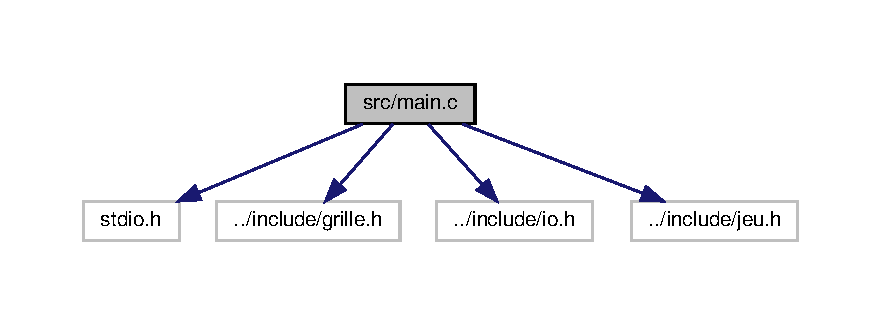
\includegraphics[width=267pt]{main_8c__incl}
\end{center}
\end{figure}
\subsection*{Functions}
\begin{DoxyCompactItemize}
\item 
int \hyperlink{main_8c_a3c04138a5bfe5d72780bb7e82a18e627}{main} (int argc, char $\ast$$\ast$argv)
\begin{DoxyCompactList}\small\item\em Fonction main classique, avec tout ses appels. \end{DoxyCompactList}\end{DoxyCompactItemize}


\subsection{Detailed Description}
Fichier \hyperlink{main_8c}{main.\+c} (coeur) 



\subsection{Function Documentation}
\index{main.\+c@{main.\+c}!main@{main}}
\index{main@{main}!main.\+c@{main.\+c}}
\subsubsection[{\texorpdfstring{main(int argc, char $\ast$$\ast$argv)}{main(int argc, char **argv)}}]{\setlength{\rightskip}{0pt plus 5cm}int main (
\begin{DoxyParamCaption}
\item[{int}]{argc, }
\item[{char $\ast$$\ast$}]{argv}
\end{DoxyParamCaption}
)}\hypertarget{main_8c_a3c04138a5bfe5d72780bb7e82a18e627}{}\label{main_8c_a3c04138a5bfe5d72780bb7e82a18e627}


Fonction main classique, avec tout ses appels. 

\begin{DoxyReturn}{Returns}
0 
\end{DoxyReturn}

%--- End generated contents ---

% Index
\backmatter
\newpage
\phantomsection
\clearemptydoublepage
\addcontentsline{toc}{chapter}{Index}
\printindex

\end{document}
